\documentclass[aspectratio=169, table]{beamer}

%\usepackage[beamertheme=./praditatheme]{Pradita}
\usepackage[utf8]{inputenc}
\usepackage{xcolor} % for color
\usepackage{colortbl} % for table color
\usepackage{listings}

% Define Java language style for listings
\lstdefinestyle{JavaStyle}{
language=Java,
basicstyle=\ttfamily\scriptsize,
keywordstyle=\color{blue},
commentstyle=\color{gray},
stringstyle=\color{red},
breaklines=true,
showstringspaces=false,
tabsize=2,
captionpos=b,
numbers=left,
numberstyle=\tiny\color{gray},
frame=lines,
backgroundcolor=\color{lightgray!10},
comment=[l]{//},
morecomment=[s]{/*}{*/},
commentstyle=\color{gray}\ttfamily,
string=[s]{'}{'},
morestring=[s]{"}{"},
%	stringstyle=\color{teal}\ttfamily,
%	showstringspaces=false
}

%
%\lstdefinestyle{sql}{
%language=sql,
%keywords={use, insert, into, values, select, from,
%update, set, delete, create, where, join, left, right, inner, order, by, primary, key},
%ndkeywords={max, min, varchar, int},
%ndkeywordstyle=\color{purple}\bfseries,
%basicstyle=\ttfamily\scriptsize,
%keywordstyle=\color{blue},
%commentstyle=\color{gray},
%stringstyle=\color{red},
%breaklines=true,
%showstringspaces=false,
%tabsize=2,
%captionpos=b,
%numbers=left,
%numberstyle=\tiny\color{gray},
%frame=lines,
%backgroundcolor=\color{lightgray!10},
%comment=[l]{\#},
%morecomment=[s]{/*}{*/},
%commentstyle=\color{gray}\ttfamily,
%string=[s]{'}{'},
%morestring=[s]{"}{"},
%%	stringstyle=\color{teal}\ttfamily,
%%	showstringspaces=false
%}
%
%\lstdefinelanguage{bash} {
%keywords={},
%basicstyle=\ttfamily\scriptsize,
%keywordstyle=\color{blue}\bfseries,
%ndkeywords={iex},
%ndkeywordstyle=\color{purple}\bfseries,
%sensitive=true,
%commentstyle=\color{gray},
%stringstyle=\color{red},
%numbers=left,
%numberstyle=\tiny\color{gray},
%breaklines=true,
%frame=lines,
%backgroundcolor=\color{lightgray!10},
%tabsize=2,
%comment=[l]{\#},
%morecomment=[s]{/*}{*/},
%commentstyle=\color{gray}\ttfamily,
%stringstyle=\color{purple}\ttfamily,
%showstringspaces=false
%}
%
%\lstdefinestyle{XmlStyle} {
%language=xml,
%keywords={xmlns,version,type,import},
%basicstyle=\ttfamily\scriptsize,
%keywordstyle=\color{blue}\bfseries,
%ndkeywords={import},
%ndkeywordstyle=\color{purple}\bfseries,
%sensitive=true,
%commentstyle=\color{gray},
%stringstyle=\color{red},
%numbers=left,
%numberstyle=\tiny\color{gray},
%breaklines=true,
%frame=lines,
%backgroundcolor=\color{lightgray!10},
%tabsize=2,
%showstringspaces=false,
%comment=[l]{\#},
%commentstyle=\color{gray}\ttfamily,
%stringstyle=\color{purple}\ttfamily,
%morecomment=[s]{<!--}{-->}
%}
%
%\lstdefinelanguage{css}{
%basicstyle=\ttfamily\footnotesize,
%keywordstyle=\color{blue},
%commentstyle=\color{gray},
%stringstyle=\color{red},
%breaklines=true,
%showstringspaces=false,
%tabsize=2,
%captionpos=b,
%numbers=left,
%numberstyle=\tiny\color{gray},
%frame=lines,
%backgroundcolor=\color{lightgray!10},
%comment=[l]{//},
%morecomment=[s]{/*}{*/},
%commentstyle=\color{gray}\ttfamily,
%string=[s]{'}{'},
%morestring=[s]{"}{"},
%%	stringstyle=\color{teal}\ttfamily,
%%	showstringspaces=false
%}
%
%\lstdefinelanguage{puml}{
%	basicstyle=\ttfamily\footnotesize,
%	keywords={@startuml, @enduml, class, String, abstract, interface, Person, note, of, end, enum},
%	ndkeywords={right, left},
%	morekeywords={\{,\}, <!-- },
%	emph={=,!,?}, emphstyle=\color{red}\bfseries,
%	keywordstyle=\color{blue},
%	commentstyle=\color{gray},
%	stringstyle=\color{teal},
%	ndkeywordstyle=\color{purple}\bfseries,
%	breaklines=true,
%	showstringspaces=false,
%	tabsize=2,
%	captionpos=b,
%	numbers=left,
%	numberstyle=\tiny\color{gray},
%	frame=lines,
%	backgroundcolor=\color{lightgray!10},
%	comment=[l]{\'},
%	morecomment=[s]{/*}{*/},
%	commentstyle=\color{gray}\ttfamily,
%	%	string=[s]{'}{'},
%	morestring=[s]{"}{"},
%	%	stringstyle=\color{teal}\ttfamily,
%	%	showstringspaces=false
%	literate=
%	{\{}{{\textcolor{red}{\{}}}1
%	{\}}{{\textcolor{red}{\}}}}1
%	{:}{{\textcolor{red}{:}}}1
%	{=}{{\textcolor{red}{=}}}1
%}

\usetheme{Pradita}
%
\subtitle{IF220303 - Object-oriented Programming}

\title{\Huge{Design Patterns \&\\\vspace{5pt}Creational Patterns}}
\date[Serial]{\scriptsize {PRU/SPMI/FR-BM-18/0222}}
\author[Pradita]{\small {\textbf{Alfa Yohannis}}}

\begin{document}

\frame{\titlepage}

\begin{frame}[fragile]
\frametitle{Contents}
\vspace{20pt}
\begin{columns}[t]
\column{0.5\textwidth}
\tableofcontents[sections={1-5}]

\column{0.5\textwidth}
\tableofcontents[sections={6-10}]
\end{columns}
\end{frame}

\section{Introduction}

\begin{frame}[fragile]{What Are Design Patterns?}
\vspace{10pt}
\begin{columns}[T]
\column{0.5\textwidth}
\textbf{Definition:}

Design patterns are proven and reusable solutions to common software design problems, especially in object-oriented development.

\vspace{8pt}
They are not final code but rather templates or blueprints that can be adapted to specific contexts.

\column{0.5\textwidth}
\textbf{Origins and Purpose:}

Patterns emerged from best practices and experiences shared by developers to build flexible, maintainable, and structured systems.

\vspace{8pt}
They help teams adopt a shared vocabulary for common challenges in software design.
\end{columns}
\end{frame}

\begin{frame}[fragile]{Design Pattern Categories}
\vspace{10pt}
\begin{columns}[T]
\column{0.5\textwidth}
\textbf{Creational Patterns}
\begin{itemize}
\item Focus on object creation
\item Improve flexibility and control
\item Examples:
\textit{Singleton, Factory Method, Abstract Factory}
\end{itemize}

\textbf{Structural Patterns}
\begin{itemize}
\item Organise class \& object structures
\item Enable scalable architecture
\item Examples:
\textit{Adapter, Composite, Decorator}
\end{itemize}

\column{0.5\textwidth}
\textbf{Behavioral Patterns}
\begin{itemize}
\item Manage object interactions
\item Simplify communication logic
\item Examples:
\textit{Strategy, Observer, Command}
\end{itemize}

\textbf{Key Point:}
\begin{itemize}
\item Categories reflect intent:
creation, structure, and behaviour
\end{itemize}
\end{columns}
\end{frame}

\begin{frame}[fragile]{Why Use Design Patterns?}
\vspace{10pt}
\begin{columns}[T]
\column{0.5\textwidth}
\textbf{Strategic Benefits}
\begin{itemize}
\item \textbf{Reusability}:
Same solution, multiple contexts
\item \textbf{Readability \& Communication}:
Named patterns improve team collaboration
\item \textbf{Architectural Consistency}:
Promotes predictable, unified design
\end{itemize}

\column{0.5\textwidth}
\textbf{Engineering Impact}
\begin{itemize}
\item \textbf{Maintainability}: Easier updates with lower risk
\item \textbf{Extensibility}: Supports Open/Closed Principle
\item \textbf{Quality \& Longevity}: Reduces code duplication and complexity
\end{itemize}

\vspace{5pt}
Design patterns enable clean, elegant, and sustainable software design.
\end{columns}
\end{frame}

\section{Creational Pattern: Singleton}

\begin{frame}[fragile]{Singleton: Goal and Use Cases}
\vspace{10pt}
\begin{columns}[T]
\column{0.5\textwidth}
\textbf{Goal:}
\begin{itemize}
\item Ensure a class has only one instance
\item Provide global access point to that instance
\end{itemize}

\textbf{Typical Uses:}
\begin{itemize}
\item Global configuration manager
\item System logger
\item Database connection manager
\item Cache controller
\end{itemize}

\column{0.5\textwidth}
\textbf{Implementation Approach:}
\begin{itemize}
\item Hide constructor using \texttt{private}
\item Provide static method to access the instance
\end{itemize}

\vspace{5pt}
Useful when multiple instances may lead to inconsistency or conflicts.
\end{columns}
\end{frame}

\begin{frame}[fragile]{Singleton: Practical Examples}
\vspace{10pt}
\begin{columns}[T]
\column{0.5\textwidth}
\textbf{Logger:}
\begin{itemize}
\item One central logger for all activities
\item Prevents unnecessary duplication
\end{itemize}

\vspace{10pt}
\textbf{Configuration Manager:}
\begin{itemize}
\item Stores paths, server addresses, network settings
\item Loaded once and shared across system
\end{itemize}

\column{0.5\textwidth}
\textbf{Pattern Characteristics:}
\begin{itemize}
\item Centralised instance management
\item Controlled lifecycle
\item Common in frameworks and platforms
\end{itemize}
\end{columns}
\end{frame}

\begin{frame}[fragile]{Singleton: Pros and Cons}
\vspace{10pt}
\begin{columns}[T]
\column{0.5\textwidth}
\textbf{Advantages:}
\begin{itemize}
\item \textbf{Controlled instance:} Only one object exists
\item \textbf{Global access:} Easy to reach from anywhere
\item \textbf{Efficient:} Saves memory and resource reuse
\end{itemize}

\column{0.5\textwidth}
\textbf{Disadvantages:}
\begin{itemize}
\item \textbf{Hard to test:} Global state hinders unit isolation
\item \textbf{Violates SRP \& DIP:} Becomes overly responsible and tightly coupled
\item \textbf{Thread safety issues:} May cause race conditions if not handled properly
\end{itemize}
\end{columns}
\end{frame}

\begin{frame}[fragile]{Singleton: Thread-Safety Pitfall}
\vspace{10pt}
\textbf{Problem:} Basic implementation fails in multithreaded environments

\begin{lstlisting}[style=JavaStyle]
public class Config {
private static Config instance;

private Config() {}

public static Config getInstance() {
	if (instance == null) {
		instance = new Config();
	}
	return instance;
}
}
\end{lstlisting}

\vspace{5pt}
Two threads may simultaneously enter \texttt{getInstance()} while \texttt{instance} is still \texttt{null}, creating two separate objects—breaking the singleton guarantee.
\end{frame}


\begin{frame}[fragile]{Java Implementation Overview}
\vspace{10pt}
\begin{columns}[T]
\column{0.5\textwidth}
\textbf{Class Diagram Summary:}
\begin{itemize}
\item Constructor \texttt{Singleton()} is \texttt{private} to prevent direct instantiation.
\item Static field \texttt{instance} holds the sole object.
\item Static method \texttt{getInstance()} gives global access.
\item Method \texttt{doSomething()} represents general operations.
\end{itemize}

\vspace{10pt}
\textbf{Purpose:} Ensure only one object is created and accessed globally across the system.

\column{0.5\textwidth}
\begin{figure}[h]
\centering
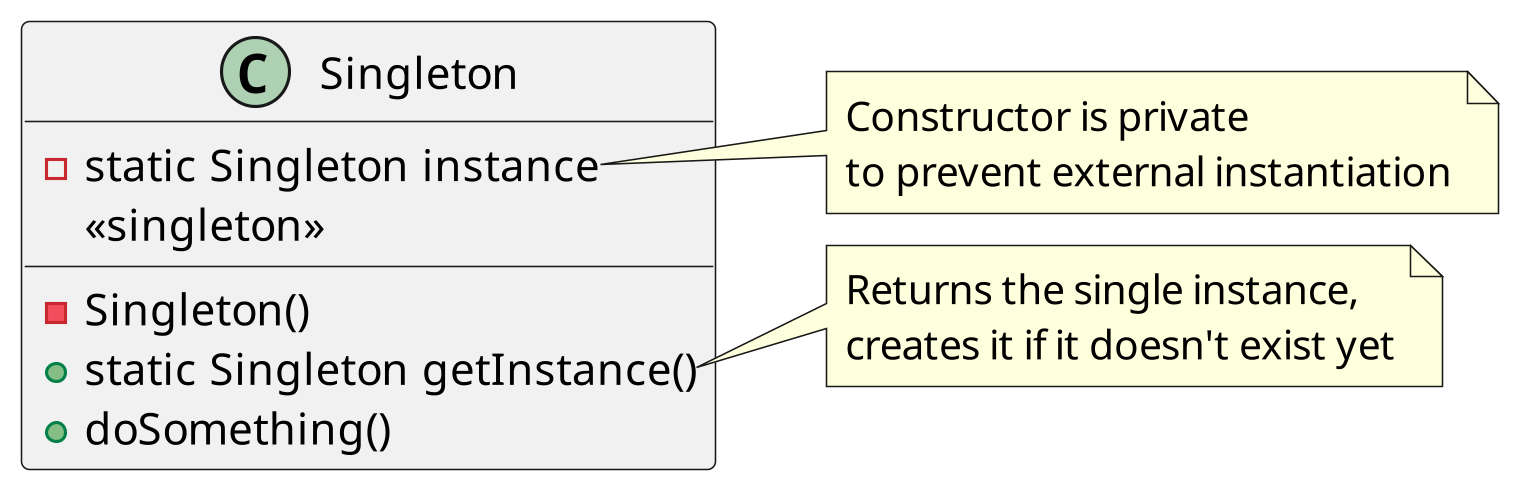
\includegraphics[width=\linewidth]{../../figures/out/singleton.png}
\end{figure}
\end{columns}
\end{frame}

\begin{frame}[fragile]{1. Simple Singleton (Not Thread-Safe)}
\vspace{5pt}
\begin{columns}[T]
\column{0.4\textwidth}
\textbf{Key Points:}
\begin{itemize}
\item Uses private constructor
\item Provides static \texttt{getInstance()} method
\item Easy to implement
\item Not safe in multithreaded environments
\end{itemize}

\textbf{Drawback:}
Two threads could both create an instance at the same time if accessed simultaneously.

\column{0.6\textwidth}
\begin{lstlisting}[style=JavaStyle]
public class SimpleSingleton {
	private static SimpleSingleton instance;
	
	private SimpleSingleton() {}
	
	public static SimpleSingleton getInstance() {
		if (instance == null) {
			instance = new SimpleSingleton();
		}
		return instance;
	}
}
\end{lstlisting}
\end{columns}
\end{frame}

\begin{frame}[fragile]{2. Thread-Safe Singleton (\texttt{synchronized})}
\vspace{5pt}
\begin{columns}[T]
\column{0.4\textwidth}
\textbf{Key Points:}
\begin{itemize}
\item Uses \texttt{synchronized} keyword
\item Prevents race conditions during first instantiation
\item Safer for concurrent use
\end{itemize}

\textbf{Trade-off:}
Synchronisation adds overhead—affects performance if called frequently.

\column{0.6\textwidth}
\begin{lstlisting}[style=JavaStyle]
public class ThreadSafeSingleton {
	private static ThreadSafeSingleton instance;
	
	private ThreadSafeSingleton() {}
	
	public static synchronized 
	ThreadSafeSingleton getInstance() {
		if (instance == null) {
			instance = new ThreadSafeSingleton();
		}
		return instance;
	}
}
\end{lstlisting}
\end{columns}
\end{frame}

\begin{frame}[fragile]{3. Double-Checked Locking}
\vspace{20pt}
\begin{columns}[T]
\column{0.35\textwidth}
\textbf{Purpose:}
\begin{itemize}
\item Combine performance and thread-safety
\item Locking only occurs on first access
\end{itemize}

\textbf{Key Technique:}
\begin{itemize}
\item Uses \texttt{volatile} for visibility across threads
\item Prevents multiple instance creation
\end{itemize}

\column{0.65\textwidth}
\begin{lstlisting}[style=JavaStyle]
public class DoubleCheckedSingleton {
	private static volatile 
	DoubleCheckedSingleton instance;
	
	private DoubleCheckedSingleton() {}
	
	public static DoubleCheckedSingleton 
	getInstance() {
		if (instance == null) {
			synchronized (DoubleCheckedSingleton.class) {
				if (instance == null) {
					instance = new DoubleCheckedSingleton();
				}
			}
		}
		return instance;
	}
}
\end{lstlisting}
\end{columns}
\end{frame}

\begin{frame}[fragile]{4. Holder Idiom (Recommended)}
\vspace{5pt}
\begin{columns}[T]
\column{0.4\textwidth}
\textbf{Advantages:}
\begin{itemize}
\item Thread-safe by JVM class loading
\item Lazy-loaded only on first use
\item No need for \texttt{synchronized}
\end{itemize}

\textbf{JVM Guarantee:}
Inner class is not loaded until referenced.

\column{0.6\textwidth}
\begin{lstlisting}[style=JavaStyle]
public class HolderSingleton {
	private HolderSingleton() {}
	
	private static class SingletonHolder {
		private static final HolderSingleton 
		INSTANCE = new HolderSingleton();
	}
	
	public static HolderSingleton getInstance() {
		return SingletonHolder.INSTANCE;
	}
}
\end{lstlisting}
\end{columns}
\end{frame}

\begin{frame}[fragile]{5. Enum-Based Singleton (Safest)}
\vspace{5pt}
\begin{columns}[T]
\column{0.45\textwidth}
\textbf{Why Use Enum:}
\begin{itemize}
\item Thread-safe by default
\item Serialization-safe
\item Easy to implement
\end{itemize}

\textbf{Limitation:}
Cannot extend other classes.

\textbf{Usage:}
\begin{lstlisting}[style=JavaStyle]
EnumSingleton.INSTANCE.doSomething();
\end{lstlisting}

\column{0.55\textwidth}
\begin{lstlisting}[style=JavaStyle]
public enum EnumSingleton {
	INSTANCE;
	
	public void doSomething() {
		System.out.println("Doing something...");
	}
}
\end{lstlisting}
\end{columns}
\end{frame}

\section{Creational Pattern: Factory Method}

\begin{frame}[fragile]{Factory Method: Purpose and Context}
\vspace{10pt}
\begin{columns}[T]
\column{0.5\textwidth}
\textbf{Goal:}
\begin{itemize}
\item Avoid direct dependency on concrete classes
\item Define a method for creating objects, but let subclasses decide which class to instantiate
\end{itemize}

\textbf{Key Use Cases:}
\begin{itemize}
\item When object type is unknown at compile time
\item When object creation requires complex logic
\item To support the Open/Closed Principle
\end{itemize}

\column{0.5\textwidth}
\textbf{Common Usage:}
\begin{itemize}
\item Frameworks define structure
\item Developers provide specific implementations via subclassing
\end{itemize}

\vspace{5pt}
Useful for building extensible and decoupled systems.
\end{columns}
\end{frame}

\begin{frame}[fragile]{Factory Method: Real-World Examples}
\vspace{10pt}
\begin{columns}[T]
\column{0.5\textwidth}
\textbf{Example: GUI Framework}
\begin{itemize}
\item Abstract \texttt{Dialog} class defines \texttt{createButton()}
\item \texttt{WindowsDialog} returns \texttt{WindowsButton}
\item \texttt{LinuxDialog} returns \texttt{LinuxButton}
\end{itemize}

\textbf{Benefit:}
Each platform defines its own button creation without altering the client code

\column{0.5\textwidth}
\textbf{Example: Transport Ordering System}
\begin{itemize}
\item Abstract \texttt{TransportFactory} defines \texttt{createTransport()}
\item \texttt{CarFactory} creates \texttt{Car}
\item \texttt{BikeFactory} creates \texttt{Bike}
\end{itemize}

\textbf{Benefit:}
Client remains unaware of specific product classes
\end{columns}
\end{frame}

\begin{frame}[fragile]{Factory Method: Pros and Cons}
\vspace{10pt}
\begin{columns}[T]
\column{0.5\textwidth}
\textbf{Advantages:}
\begin{itemize}
\item \textbf{Flexible \& Extensible:} Add new products via subclassing
\item \textbf{Supports SOLID:} Aligns with Open/Closed and Dependency Inversion
\item \textbf{Cleaner client code:} No need to know concrete classes
\end{itemize}

\column{0.5\textwidth}
\textbf{Disadvantages:}
\begin{itemize}
\item \textbf{Increased complexity:} Requires many subclasses
\item \textbf{Harder to read:} Interface and hierarchy separation may confuse beginners
\item \textbf{Overkill for simple cases:} Unnecessary when only a few object types are needed
\end{itemize}
\end{columns}
\end{frame}

\begin{frame}[fragile]{Java Code: Factory Method Overview}
\vspace{5pt}
\begin{columns}[T]
\column{0.5\textwidth}
\textbf{Concept:}
\begin{itemize}
\item Abstract class defines factory method
\item Subclasses decide which concrete object to create
\item Client works with interface, not implementation
\end{itemize}

\textbf{Goal:} Decouple object creation from usage

\vspace{5pt}
\textbf{Use Case:} Transport system supporting car and bike

\column{0.5\textwidth}
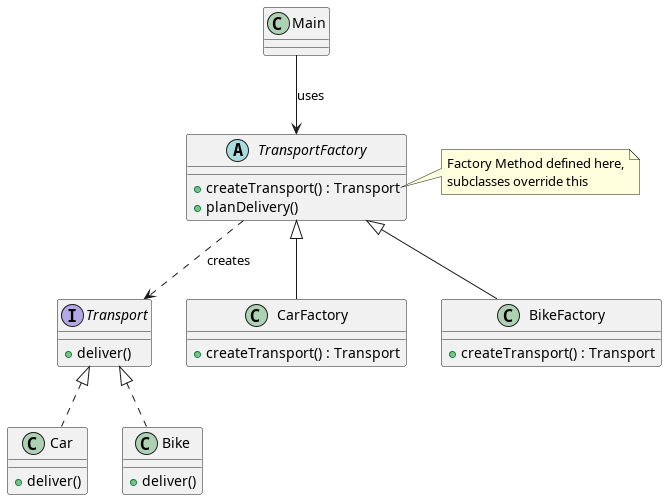
\includegraphics[width=\linewidth]{../../figures/out/factory_method.png}
\end{columns}
\end{frame}

\begin{frame}[fragile]{Step 1: Product Interface \& Implementations}
\vspace{5pt}
\begin{columns}[T]
\column{0.65\textwidth}
\begin{lstlisting}[style=JavaStyle]
// Product interface
public interface Transport {
	void deliver();
}

// Concrete products
public class Car implements Transport {
	public void deliver() {
		System.out.println("Delivery by car.");
	}
}

public class Bike implements Transport {
	public void deliver() {
		System.out.println("Delivery by bike.");
	}
}
\end{lstlisting}

\column{0.35\textwidth}
\begin{itemize}
\item \texttt{Transport} defines a unified delivery behaviour.
\item \texttt{Car} and \texttt{Bike} implement this interface.
\item Promotes consistency and abstraction across transport types.
\end{itemize}
\end{columns}
\end{frame}

\begin{frame}[fragile]{Step 2: Abstract Factory}
\vspace{5pt}
\begin{columns}[T]
\column{0.65\textwidth}
\begin{lstlisting}[style=JavaStyle]
// Abstract creator with factory method
public abstract class TransportFactory {
	public abstract Transport createTransport();
	
	public void planDelivery() {
		Transport transport = createTransport();
		transport.deliver();
	}
}
\end{lstlisting}

\column{0.35\textwidth}
\begin{itemize}
\item \texttt{createTransport()} is the factory method.
\item \texttt{planDelivery()} defines a fixed algorithm.
\item The concrete object is determined by subclasses.
\end{itemize}
\end{columns}
\end{frame}

\begin{frame}[fragile]{Step 3: Concrete Factories}
\vspace{5pt}
\begin{columns}[T]
\column{0.65\textwidth}
\begin{lstlisting}[style=JavaStyle]
public class CarFactory extends TransportFactory {
	public Transport createTransport() {
		return new Car();
	}
}

public class BikeFactory extends TransportFactory {
	public Transport createTransport() {
		return new Bike();
	}
}
\end{lstlisting}

\column{0.35\textwidth}
\begin{itemize}
\item Each subclass defines the transport it creates.
\item Enables switching types without touching core logic.
\item Encourages extension with minimal modification.
\end{itemize}
\end{columns}
\end{frame}

\begin{frame}[fragile]{Step 4: Client Code}
\vspace{5pt}
\begin{columns}[T]
\column{0.65\textwidth}
\begin{lstlisting}[style=JavaStyle]
public class Main {
	public static void main(String[] args) {
		TransportFactory factory;
		
		factory = new CarFactory();
		factory.planDelivery(); // Delivery by car.
		
		factory = new BikeFactory();
		factory.planDelivery(); // Delivery by bike.
	}
}
\end{lstlisting}

\column{0.35\textwidth}
\begin{itemize}
\item Client only depends on the abstract factory.
\item No need to modify client logic to support new types.
\item Supports Open/Closed Principle effectively.
\end{itemize}
\end{columns}
\end{frame}


\begin{frame}[fragile]{Discussion and Design Impact}
\vspace{5pt}
\begin{columns}[T]
\column{0.5\textwidth}
\textbf{SOLID Support:}
\begin{itemize}
\item \textbf{Open/Closed}: Extendable via new factories
\item \textbf{DIP}: Depends on \texttt{Transport} interface
\end{itemize}

\textbf{Framework Friendly:}
\begin{itemize}
\item Framework defines the structure
\item Developers inject specific behaviour via subclassing
\end{itemize}

\column{0.5\textwidth}
\textbf{Benefits:}
\begin{itemize}
\item Clear separation between creator and product
\item Improved modularity and testability
\end{itemize}

\textbf{Trade-offs:}
\begin{itemize}
\item Adds class hierarchy complexity
\item May feel over-engineered for simple needs
\end{itemize}
\end{columns}
\end{frame}


\section{Creational Pattern: Abstract Factory}

\begin{frame}[fragile]{Abstract Factory: Purpose and Context}
\vspace{5pt}
\begin{columns}[T]
\column{0.5\textwidth}
\textbf{Purpose:}
\begin{itemize}
\item Provide an interface for creating families of related objects.
\item Clients do not depend on specific concrete classes.
\item Ensure compatibility between objects created by the same factory.
\end{itemize}

\column{0.5\textwidth}
\textbf{Common Use Cases:}
\begin{itemize}
\item Systems that support multiple configurations or themes.
\item Object creation involves complex interdependencies.
\item Easily switch object families without modifying main code.
\end{itemize}
\end{columns}
\end{frame}

\begin{frame}[fragile]{Use Case 1: Cross-Platform GUI Toolkit}
\vspace{5pt}
\begin{columns}[T]
\column{0.5\textwidth}
\textbf{Example: GUI Abstraction}
\begin{itemize}
\item Products: \texttt{Button}, \texttt{Checkbox}
\item Windows: \texttt{WinButton}, \texttt{WinCheckbox}
\item macOS: \texttt{MacButton}, \texttt{MacCheckbox}
\end{itemize}

\column{0.5\textwidth}
\textbf{Benefits:}
\begin{itemize}
\item Change theme by switching factory
\item No changes required in application logic
\item Supports consistent user interface design
\end{itemize}
\end{columns}
\end{frame}

\begin{frame}[fragile]{Use Case 2: Multi-Database Support}
\vspace{5pt}
\begin{columns}[T]
\column{0.5\textwidth}
\textbf{Example: Database Toolkit}
\begin{itemize}
\item Products: \texttt{Connection}, \texttt{QueryBuilder}
\item Factories: \texttt{MySQLFactory}, \texttt{PostgresFactory}, \texttt{OracleFactory}
\end{itemize}

\column{0.5\textwidth}
\textbf{Advantages:}
\begin{itemize}
\item Vendor-specific implementations are encapsulated
\item Switching backend only requires changing the factory
\item Promotes code reuse and isolation
\end{itemize}
\end{columns}
\end{frame}

\begin{frame}[fragile]{Benefits of Abstract Factory}
\vspace{5pt}
\begin{columns}[T]
\column{0.5\textwidth}
\textbf{1. Product Consistency}
\begin{itemize}
\item Ensures all UI components belong to the same design system
\item \textit{e.g.} \texttt{WinFactory} ensures all widgets match Windows style
\end{itemize}

\textbf{2. SOLID Principles}
\begin{itemize}
\item Supports \textbf{DIP}: Client depends on abstraction
\item Supports \textbf{OCP}: Add new families via new factories
\end{itemize}

\column{0.5\textwidth}
\textbf{3. No Concrete Class Coupling}
\begin{itemize}
\item Clients don’t need to know specific implementations
\item \texttt{factory.createButton()} hides whether it’s Mac or Win
\end{itemize}

\textbf{4. Easy Reconfiguration}
\begin{itemize}
\item Switch entire look-and-feel with one factory instance
\item \textit{e.g.} switch to \texttt{DarkThemeFactory} to enable dark mode
\end{itemize}
\end{columns}
\end{frame}

\begin{frame}[fragile]{Drawbacks of Abstract Factory}
\vspace{5pt}
\begin{columns}[T]
\column{0.5\textwidth}
\textbf{1. Class Explosion}
\begin{itemize}
\item Requires many interfaces and classes
\item \textit{e.g.} 3 variants × 2 products = 9+ classes/interfaces
\end{itemize}

\textbf{2. Overhead for Simple Cases}
\begin{itemize}
\item Not ideal if only one component type varies
\item \textit{e.g.} replacing just \texttt{Button} doesn’t need a full factory
\end{itemize}

\column{0.5\textwidth}
\textbf{3. High Abstraction Barrier}
\begin{itemize}
\item Involves composition of multiple design patterns
\item Difficult for beginners to understand the structure
\item Requires knowledge of interfaces, inheritance, and delegation
\end{itemize}
\end{columns}
\end{frame}


\begin{frame}[fragile]{Abstract Factory: Implementation Overview}
\vspace{5pt}
\begin{columns}[T]
\column{0.5\textwidth}
\textbf{Overview:}
\begin{itemize}
\item Interface-based product family: \texttt{Button}, \texttt{Checkbox}
\item \texttt{GUIFactory} defines creation of both
\item Concrete factories: \texttt{WinFactory}, \texttt{MacFactory}
\end{itemize}

\column{0.5\textwidth}
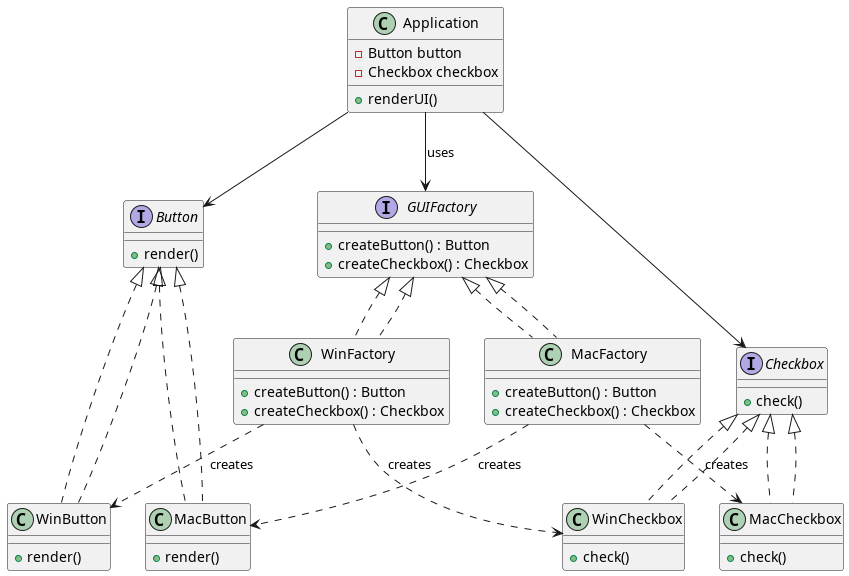
\includegraphics[width=\linewidth]{../../figures/out/factory_abstract.png}
\end{columns}
\end{frame}

\begin{frame}[fragile]{Step 1: Interfaces \& Implementations}
\vspace{20pt}
\begin{columns}[T]
\column{0.65\textwidth}
\begin{lstlisting}[style=JavaStyle]
// Product 1: Button
public interface Button {
	void render();
}

public class WinButton implements Button {
	public void render() {
		System.out.println("Render Windows-style button.");
	}
}

public class MacButton implements Button {
	public void render() {
		System.out.println("Render macOS-style button.");
	}
}
\end{lstlisting}

\column{0.35\textwidth}
\begin{itemize}
\item \texttt{Button} defines the abstraction.
\item Concrete implementations render platform-specific styles.
\item Allows interchangeable use in UI code.
\end{itemize}
\end{columns}
\end{frame}

\begin{frame}[fragile]{Step 2: Second Product Family: Checkbox}
\vspace{20pt}
\begin{columns}[T]
\column{0.65\textwidth}
\begin{lstlisting}[style=JavaStyle]
// Product 2: Checkbox
public interface Checkbox {
	void check();
}

public class WinCheckbox implements Checkbox {
	public void check() {
		System.out.println("Check Windows-style checkbox.");
	}
}

public class MacCheckbox implements Checkbox {
	public void check() {
		System.out.println("Check macOS-style checkbox.");
	}
}
\end{lstlisting}

\column{0.35\textwidth}
\begin{itemize}
\item Abstracts checkbox logic for different platforms.
\item Follows the same structure as the button product.
\item Consistent usage across the client.
\end{itemize}
\end{columns}
\end{frame}

\begin{frame}[fragile]{Step 3: Abstract Factory Interface}
\vspace{5pt}
\begin{columns}[T]
\column{0.65\textwidth}
\begin{lstlisting}[style=JavaStyle]
// Abstract Factory
public interface GUIFactory {
	Button createButton();
	Checkbox createCheckbox();
}
\end{lstlisting}

\column{0.35\textwidth}
\begin{itemize}
\item Common interface to produce product families.
\item Client interacts only with this factory.
\item Promotes consistency and abstraction.
\end{itemize}
\end{columns}
\end{frame}

\begin{frame}[fragile]{Step 4: Concrete Factories}
\vspace{20pt}
\begin{columns}[T]
\column{0.65\textwidth}
\begin{lstlisting}[style=JavaStyle]
// Windows variant
public class WinFactory implements GUIFactory {
	public Button createButton() {
		return new WinButton();
	}
	public Checkbox createCheckbox() {
		return new WinCheckbox();
	}
}

// macOS variant
public class MacFactory implements GUIFactory {
	public Button createButton() {
		return new MacButton();
	}
	public Checkbox createCheckbox() {
		return new MacCheckbox();
	}
}
\end{lstlisting}

\column{0.35\textwidth}
\begin{itemize}
\item Each factory produces compatible product sets.
\item Switching factories changes the full UI theme.
\item Supports platform scalability.
\end{itemize}
\end{columns}
\end{frame}

\begin{frame}[fragile]{Step 5: Client Code with Abstract Factory}
\vspace{30pt}
\begin{columns}[T]
\column{0.65\textwidth}
\begin{lstlisting}[style=JavaStyle]
public class Application {
	private Button button;
	private Checkbox checkbox;
	public Application(GUIFactory factory) {
		button = factory.createButton();
		checkbox = factory.createCheckbox();
	}
	public void renderUI() {
		button.render();
		checkbox.check();
	}
	public static void main(String[] args) {
		GUIFactory factory;
		factory = new WinFactory();
		Application app1 = new Application(factory);
		app1.renderUI();
		factory = new MacFactory();
		Application app2 = new Application(factory);
		app2.renderUI();
	}
}
\end{lstlisting}

\column{0.35\textwidth}
\begin{itemize}
\item Client depends only on \texttt{GUIFactory}.
\item Easily change style without altering core logic.
\item Greatly simplifies code maintenance and testing.
\end{itemize}
\end{columns}
\end{frame}

\begin{frame}[fragile]{Discussion: Design Structure and Benefits}
\vspace{5pt}
\begin{columns}[T]
\column{0.5\textwidth}
\textbf{What This Structure Provides:}
\begin{itemize}
\item Full abstraction from platform-specific UI code.
\item Reusable logic for rendering and interaction.
\item Easy testing and swapping of factories.
\end{itemize}

\column{0.5\textwidth}
\textbf{Resulting Benefits:}
\begin{itemize}
\item Highly modular and scalable architecture.
\item Supports Open/Closed and Dependency Inversion.
\item Facilitates theme-switching and platform adaptation.
\end{itemize}
\end{columns}
\end{frame}

\begin{frame}[fragile]{Conceptual Explanation}
	\vspace{20pt}
	\begin{columns}[T]
		\column{0.5\textwidth}
		\textbf{Factory Method}
		\begin{itemize}
			\item Provides a single method like \texttt{createProduct()}.
			\item Subclasses decide which concrete object is created.
			\item Focus: Flexibility and delegation to subclasses.
			\item Suitable for when you need to instantiate one type of object.
		\end{itemize}
		\textit{Example:} \texttt{CarFactory} and \texttt{BikeFactory} implement \texttt{createTransport()}.
		
		\column{0.5\textwidth}
		\textbf{Abstract Factory}
		\begin{itemize}
			\item Groups related factory methods together.
			\item Each concrete factory creates a full family of compatible objects.
			\item Focus: Consistency and product compatibility.
		\end{itemize}
		\textit{Example:} \texttt{GUIFactory} defines \texttt{createButton()}, \texttt{createCheckbox()};  
		\texttt{WinFactory} and \texttt{MacFactory} implement them consistently.
	\end{columns}
\end{frame}

\begin{frame}[fragile]{Factory Method vs Abstract Factory}
	\vspace{20pt}
	\centering
	\scriptsize
	
	\arrayrulecolor{black} % border color
	\setlength{\arrayrulewidth}{0.5pt} % thin border lines
	\rowcolors{2}{gray!10}{white}
	\begin{tabular}{|p{0.16\textwidth}|p{0.28\textwidth}|p{0.45\textwidth}|}
		\hline
		\rowcolor{gray!20} 
		\textbf{Aspect} & \textbf{Factory Method} & \textbf{Abstract Factory} \\
		\hline
		Purpose & Define concrete object in subclass & Create a family of related, compatible products \\
		\hline
		Product Type & Single product & Multiple related products \\
		\hline
		Structure & One factory method & Multiple factory methods in one interface \\
		\hline
		Number of Products & Usually one & Multiple (higher complexity) \\
		\hline
		Product Polymorphism & One hierarchy & Multiple hierarchies \\
		\hline
		Client Dependency & On one abstract product & On multiple abstract products \\
		\hline
		Common Example & \texttt{createTransport()} & \texttt{createButton()}, \texttt{createCheckbox()} \\
		\hline
		Complexity & Simpler & More complex \\
		\hline
	\end{tabular}
\end{frame}


\begin{frame}[fragile]{When to Use Each Pattern}
	\vspace{20pt}
	\begin{columns}[T]
		\column{0.5\textwidth}
		\textbf{Use Factory Method when:}
		\begin{itemize}
			\item You need to create only one type of object.
			\item You want to defer or vary object instantiation in subclasses.
			\item You prefer minimal structure and lower complexity.
		\end{itemize}
		\textit{Example:} Choosing \texttt{Car} or \texttt{Bike} at runtime via \texttt{createTransport()}.
		
		\column{0.5\textwidth}
		\textbf{Use Abstract Factory when:}
		\begin{itemize}
			\item The system requires several related objects.
			\item You want to enforce consistency across product families.
			\item You need to switch entire configurations (e.g., light/dark theme).
		\end{itemize}
		\textit{Example:} Replacing all UI components by changing from \texttt{WinFactory} to \texttt{MacFactory}.
	\end{columns}
\end{frame}

\section{Conclusion}

\begin{frame}[fragile]{Conclusion}
	\vspace{20pt}
	This chapter introduced three essential creational patterns:
	
	\vspace{10pt}
	\begin{itemize}
		\item \textbf{Singleton}: Guarantees a single global instance.
		\item \textbf{Factory Method}: Defers object creation to subclasses.
		\item \textbf{Abstract Factory}: Creates families of related objects consistently.
	\end{itemize}
	
	\vspace{10pt}
	These patterns support modularity, consistency, and key design principles like dependency inversion and scalability. Choosing the right pattern depends on the system’s context and architectural goals.
\end{frame}


\end{document}
